%! Author = dylan
%! Date = 24/03/2023

% Preamble
\documentclass[11pt]{article}

% Packages
\usepackage{geometry}
\usepackage{cite}
\usepackage{hyperref}
\usepackage{booktabs}
\usepackage{charter}
\usepackage{float}
\usepackage{listing}
\usepackage{graphicx}
\usepackage{listings}
\usepackage[dvipsnames]{xcolor}
\usepackage{fancyhdr}
\usepackage{refcount}
\usepackage[parfill]{parskip}
\usepackage[inline]{enumitem}
\usepackage{minted}

\geometry{
    a4paper,
    margin=25mm
}

\pagestyle{fancy}

\lhead{CSC4006: Research and Development Project}
\rhead{Software Development Report}
\lfoot{Dylan Wilson}
\rfoot{Queen's University Belfast}

\renewcommand{\footrulewidth}{0.4pt}

\setlength{\headheight}{15pt}

\NewDocumentCommand{\codeword}{v}{%
    \texttt{\textcolor{blue}{#1}}%
}

\patchcmd{\thebibliography}{\section*{\refname}}{}{}{}

\graphicspath{ {./images/} }

\usemintedstyle{monokai}
\definecolor{bg}{HTML}{282828}

% Document
\begin{document}

    \begin{titlepage}
        \begin{center}
            \Large
            CSC4006: Research and Development Project

            \vfill
            \Huge
            \textbf{Software Development Report}

            \medskip
            \Large
            GitSlice: Slicing the repository that feeds us

            \medskip
            by Dylan Wilson

            \vfill
            \normalsize
            \textsc{Development Repository}

            \url{https://gitlab.dylanwilson.dev/qub/csc4006-project}

            \medskip
            \textsc{EEECS Repository}

            \url{https://gitlab.eeecs.qub.ac.uk/40234266/csc4006-project}

            \medskip
            \textsc{Documentation}

            \url{https://gitslice.dylanwilson.dev/}
        \end{center}
    \end{titlepage}

    \tableofcontents

    \section{Introduction}
    \label{sec:introduction}

    This document describes usage and technical implementation details of GitSlice.
    ~\cite{gitlab} contains the source code for GitSlice.
    GitSlice is licensed under the GNU General Public License version 3.0 (commonly called GPLv3).
    The software has been developed in Python and runs using Python 3.10---although it likely will run correctly on older versions of Python as it does not make use of any particularly new language features.

    GitSlice is a tool for performing analysis on many commits of a project.
    In short, a commit in Git is a ``checkpoint'' containing some information about changes since the last commit.
    Each commit points to zero or more ``parent commits'' and describes changes since this commit.
    From this, we can build a filesystem to produce how the project looked at that specific commit.
    GitSlice iterates through these commits and selects a subset of them (based on the configuration file) for analysis.
    Some use cases for this include static code analysis and code coverage across the entire commit tree.
    The \codeword{git-rev-list} command is used for listing the commits in the repository and GitSlice allows arguments to be passed directly to \codeword{git-rev-list} (see \autoref{subsec:configuration}).

    GitSlice supports parallel and distributed execution---that is, it can run on many nodes simultaneously and on each node, multiple executions can run simultaneously (defined as a ``task'').
    More information on how this works is provided in \autoref{subsubsec:mpi}.
    
    We will begin by looking at how to configure and use GitSlice before delving into a technical description of how GitSlice works including some important dependencies of GitSlice which are required during its execution followed by a brief discussion of how it runs on the Kelvin 2 cluster specifically (in particular how it's SLURM scripts work).

    Some explicit definition of terminology is required for clarity.
    Herein, a single running version of GitSlice on a node is referred to as an instance.
    That is, when GitSlice is running on 5 nodes we will say there are 5 instances of GitSlice.
    An ``run'' of GitSlice by contrast refers to a single invocation across all nodes, regardless of how many nodes it is running.
    For example, we might say that a run of GitSlice contains 5 instances.
    The ``primary instance'' refers to the instance which is responsible for selecting commits for analysis before beginning analysis and ``secondary instances'' are only responsible for receiving commits and performing analysis on them.
    An important point to note here is the primary instance also performs analysis, but it has the additional task of identifying the commits to analyse.

    A ``version'' or ``commit'' refers to the specific set of files which existed in the repository at a particular commit.
    The ``repository'' is the repository which GitSlice is performing analysis on---when referring to the repository containing the code for GitSlice itself, this is referred to as the GitSlice repository specifically.

    The analysis tool is the tool which is providing useful information about the version---for example, generating code coverage reports or performing static code analysis.
    The analysis command is the command which invokes the analysis tool and, similarly, the analysis image is the container which contains the analysis tool.
    An ``analysis'' is a single invocation of the analysis tool on a specific version---there is always the same amount of analyses in a run of GitSlice as the amount of commits in the subset of commits selected for analysis.

    \section{Purpose, operation and validation}
    \label{sec:purpose-operation-and-validation}

    \subsection{Command-line arguments}
    \label{subsec:command-line-arguments}

    GitSlice is configured using a config file written using YAML syntax, which is given as a command-line argument.
    As of GitSlice's configuration lives within the configuration file, there are only three command-line arguments---the config file, the logging level and if dry run is enabled.

    \begin{itemize}
        \item \codeword{-l [int]}, \codeword{--log-level [int]}: The log level is given as an integer between 0 and 50, see \autoref{subsec:python-script} for more information on logging levels.
              The default log level when this argument is not supplied is \codeword{20}.
        \item \codeword{-d}, \codeword{--dry-run}: When dry run is enabled, no analysis is performed but rather the repository is cloned and the commits which would have been selected for analysis are output along with the image and command which would have been used.
              This is useful for verifying a configuration file before performing a full analysis.
              This argument does not accept any value, when it is supplied dry run mode is enabled and when it is not supplied dry run mode is disabled.
        \item \codeword{-c [str]}, \codeword{--config-file [str]}: All other configuration of the application occurs inside the configuration file.
              Specific configuration files used in the collection of data for the research article are provided in the Git repository in the config directory at~\cite{config_files}.
              The contents of this file are described in \autoref{subsec:configuration}.
    \end{itemize}

    \subsection{Configuration}
    \label{subsec:configuration}

    This section explores the configuration options, and how to use them to configure GitSlice.
    A sample configuration file from the GitSlice repository is provided in \autoref{subsec:appendix-a:-sample-configuration-file} for reference.

    \subsubsection{Directories}
    \label{subsubsec:directories}

    \codeword{Output Directory} and \codeword{Output Format}: The \codeword{Output Directory} options gives the location to store the output from each analysis.
    This directory will contain many text files, one for each version.
    These output files are named according to the \codeword{Output Format} option, which currently supports two placeholders, \codeword{\%COMMIT\_TIME\%} and \codeword{\%COMMIT\_ID\%}.
    These placeholders are replaced by the commit time (not the authored time) and the SHA1 hash of the commit respectively.
    The default output is \codeword{\%COMMIT_TIME\%\_\%COMMIT_ID\%} which will produce files as shown in \autoref{fig:sample_output}.
    The use of the commit time is helpful to provide loose ordering of the output files as the using only the hash will produce pseudorandom ordering.
    Note this ordering is only loose because it is not necessarily the same order as the output from commands git-log as it is not necessarily the case one commit created after another appears after it in the commit tree.

    \begin{figure}[H]
        \centering
        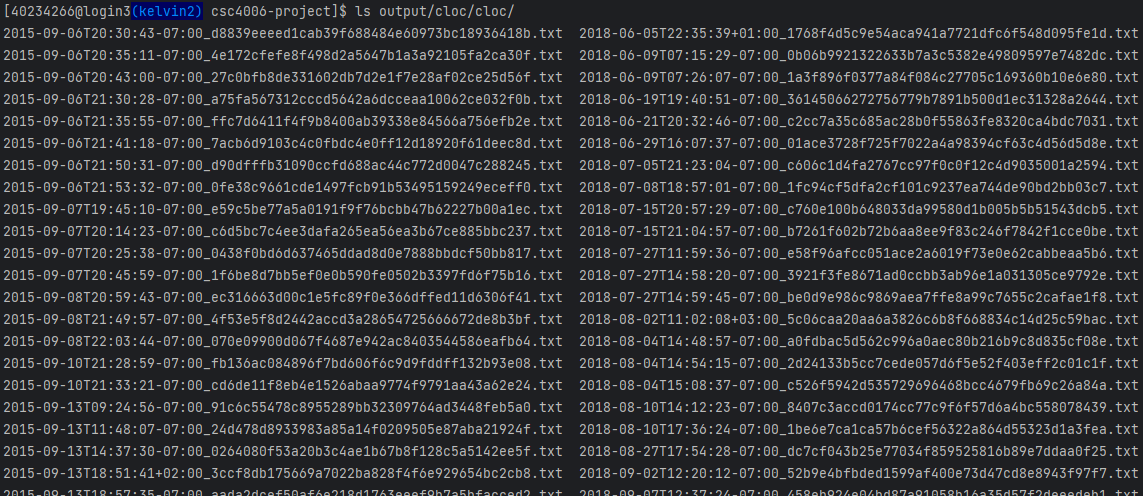
\includegraphics[width=\textwidth]{sample_output}
        \caption{Example output directory using default output format.}
        \label{fig:sample_output}
    \end{figure}

    \codeword{Temp Directory}: The \codeword{Temp Directory} options provides a temporary directory for cloning the repository to and creating the RepoFS mount in (for more information on RepoFS please see \autoref{subsubsec:repofs}).  Inside the temporary directory, each instance will create a directory for itself, these directories are named using the UUID of the instance.
    For more information on instance UUIDs see \autoref{subsubsec:mpi}.

    \codeword{Rsync To Temp}: An additional toggle, \codeword{Rsync To Temp} is also provided by GitSlice.
    This option will, when enabled, will use \codeword{rsync} to copy the files from the virtual filesystem to a directory inside the temporary directory.
    This is necessary if the analysis tool needs to modify or create files as the virtual filesystem is read-only and attempting to modify files will cause errors.
    Do note this introduces a requirement of \codeword{rsync} being available in the container.
    More information on exactly why this is necessary is provided in \autoref{subsubsec:repofs}.

    \codeword{Repo Directory Name} and \codeword{Mount Directory Name}: Finally, two options \codeword{Repo Directory Name} and \codeword{Mount Directory Name}, give the names of the directories inside the temporary directory which will be used to store a copy of the repository and the mount point for the virtual filesystem.
    This is on a per-instance basis so the final location of these directories is inside the temporary directory, inside a directory named using the UUID of the instance.
    These options are unlikely to be necessary during the execution of GitSlice (they are deleted when an instance completes and given they are inside a temporary directory used only by that instance of GitSlice, conflicts are not expected) but they are provided primarily to ensure GitSlice is fully configurable.

    \subsubsection{Git repository}

    \codeword{Git Repository Type} and \codeword{Git Repository Source}: the \codeword{Git Repository Type} option can either be \codeword{Local} or \codeword{Remote} (this option is case insensitive) and affects the expected content of the \codeword{Git Repository Source} option.
    When the repository type is \codeword{Local}, the \codeword{Git Repository Source} gives a local directory containing a Git repository which GitSlice should perform analysis on.
    When the repository type is \codeword{Remote} this should be a URL which can be used with the git-clone command - this means that any scheme such as \codeword{ssh://}, \codeword{git://}, \codeword{http[s]://} or \codeword{ftp[s]://} can be used.
    A small technical note is that when the repository option is local, the files are copied using the OS copy command, as opposed to using \codeword{git-clone} with the \codeword{--local} option.

    \codeword{Analysis}: the \codeword{Analysis} block provides the image and command which should be used.
    It is possible to use different image and commands for different versions of the project---for example, a requirements file may have been moved as some point and so a different location is needed, or an older version of the image may be needed (for example a Python project may have at one point used Python 2).
    The \codeword{Analysis} block should contain a list of commits ID and, optionally, a \codeword{Default} block.
    If the commit ID is a parent (not necessarily a direct parent, however) of the commit to be analysed, the \codeword{Image} and \codeword{Command} options under that commit will be used.
    If multiple commit IDs from the \codeword{Analysis} section are parents of the commit to be analysed, the most recent parent will be used.
    An example block is shown in \autoref{fig:analysis_configuration}.

    \begin{figure}[H]
        \centering
        \inputminted[bgcolor=bg,frame=lines,framesep=2mm]{yaml}{./listings/sample_analysis_block.yml}
        \caption{Example output directory using default output format.}
        \label{fig:analysis_configuration}
    \end{figure}

    In \autoref{fig:analysis_configuration}, GitSlice will use Python 3.8 for commits, unless they descend from \codeword{c45a101f} when Python 3.9 will be used, or if \codeword{56a676c8} is more recent then Python 3.10 will be used.
    In this example the same command is always used but this doesn't need to be the case.

    \codeword{Starting Point} and \codeword{Stopping Point}: the \codeword{Starting Point} is required but the \codeword{Stopping Point} is optional.
    Any Git object understood by \codeword{git-rev-list} can be used such as commit IDs, branches or tags.
    These options should be fairly self-explanatory---GitSlice will begin at the \codeword{Starting Point} and continue to analyse commits until it reaches the \codeword{Stopping Point} (or hits the \codeword{Commit Limit}, discussed next, or simply hits the root commit).
    When \codeword{Stopping Point} is defined, the \codeword{--ancestry-path} option is used for \codeword{git-rev-list} and the \codeword{..} operator is used, for example a \codeword{Starting Point} of \codeword{56a676c8} and \codeword{Stopping Point} of \codeword{c45a101f} will cause GitSlice to find commits using \codeword{git rev-list --ancestry-path 56a676c8..c45a101f}.

    \subsubsection{Filtering commits}

    \codeword{Git Rev List Args}: the \codeword{Git Rev List Args} option provides a list of arguments to pass to \codeword{git-rev-list}.
    This the command used by GitSlice to find commits to analyse.
    There is a great amount of flexibility in this command to select precisely which commits should be output.
    Consult the manual pages for \codeword{git-rev-list} a full description of all the options provided by this command.
    Some potentially useful options (such as \codeword{--author} and \codeword{--limit}) are described in the sample configuration files location in the \codeword{config/} directory of the GitSlice repository.
    See \autoref{subsec:appendix-a:-sample-configuration-file}, lines 115 to 133 for details.
    The content for this block is provided as keyword arguments dictionary to GitPython, so each key should be named exactly as the argument would appear in a \codeword{git-rev-list} command (without the double dash).
    Boolean options will be used without any arguments, for example \codeword{no-merges: True} will cause GitPython to use \codeword{--no-merges} where as \codeword{before: 2023-04-05T19:12:46Z} would produce \codeword{--before 2023-04-05T19:12:46Z}.
    If the value of a key is a list, then the argument will appear multiple times for example \codeword{author: ['jeff@amazon.com', 'sergey@cs.stanford.edu']} would produce \codeword{--author jeff@amazon.com --author sergey@cs.stanford.edu}.
    
    \section{Design and implementation}
    \label{sec:design-and-implementation}

    \subsection{Key dependencies}
    \label{subsec:key-dependencies}

    \subsubsection{Singularity}
    \label{subsubsec:singularity}

    One important dependency of GitSlice is Singularity, a container platform designed for use in high-performance computing environments.
    Singularity is used to run the analysis command, this allows for much greater support of potential analysis program than what would typically be support on Kelvin---in effect, any application which can be successfully containerised can be use to perform analysis across a repository using GitSlice.
    Singularity provides support for Docker containers which additionally enables support for applications which have already been containerised without the need to build the container from scratch.

    Singularity does not, however, operate similarly to Docker (at least by default).
    Importantly, Singularity containers behave more akin to natively installed programs than Docker containers---for example, Docker containers do not by default share any aspect of their filesystems with the host, and essentially operate as a lightweight virtual machine (the kernel is shared, a key difference to virtual machines but from the perspective of a running program very little is known about the outside environment).
    Singularity, however, by default will mount many of the hosts directories on the container (for example, home, and tmp directories are mounted by default).
    Furthermore, singularity shares process IDs (an ID allocated to each running process on a UNIX-based machine), and environment variables among other aspects of the host.
    The sharing of filesystems and environment variables are of particular importance here because GitSlice runs many copies of different versions of a program which can cause problems if files and variable are shared.
    For example, a Python program will have many dependencies defined as part of a requirements file of which the required version almost certainly will have changed over time---if the \codeword{PYTHONHOME} variable is set to the user's home directory (which is the case on Kelvin), each version of the application to be analysed will attempt to use whichever version of the dependency is currently available on the host which means older code may attempt to use since removed functions and classes.

    All of this to say, it is important to isolate the application from all other running versions of the application.
    Luckily, this is relatively easily done as Singularity provides an option to contain the container.
    This, however, presents a secondary issue that singularity containers are built with a filesystem with a predefined amount of disk space---specifically enough to contain the filesystem plus a small buffer amount.
    We could increase this amount of space, but it's difficult to know how much will be required, and as such it is better to mount of the scratch space onto the container.
    Disk space is also complicated by the fact RepoFS (introduced in \autoref{subsubsec:repofs}) introduces a read-only filesystem, file can instead be copied to the scratch disk if they are to be modified, the specifics of this feature are given in \autoref{subsubsec:directories} under \codeword{Rsync To Temp}.

    GitSlice communicates with Singularity on the node using the \codeword{spython} package.

    \subsubsection{RepoFS}
    \label{subsubsec:repofs}

    To avoid copying the repository many times for each thread, GitSlice uses RepoFS to bring up virtual filesystem which represents the Git repository.
    This allows the files as they existed at that commits to be mounted on the container (explained in \autoref{subsubsec:singularity}) without needing to make a copy of the repository and checkout the specific commit.
    RepoFS is a written in Python and provided using \codeword{pip} however it is not included as part of the main GitSlice script as it is run as a command via the terminal.
    This is done through a script called fsUp.sh which is called by the main GitSlice Python script.
    The similar script, fsDown.sh is called at the end of execution to bring the virtual filesystem back down.
    Occasionally, if GitSlice doesn't complete successfully this filesystem can be left---in such case a script to clean up all nodes on Kelvin from these left over mounts if provided (more information on this script is provided in \autoref{subsec:miscellaneous-scripts}).

    RepoFS requires the \codeword{libgit2} C library for calling Git's core methods.
    \codeword{libgit2} is not available on Kelvin and without permissions to install it as a system package, it needs to be installed locally by compiling it from source.
    It can prove to be slightly fiddly to ensure RepoFS is able to find the compiled files and to ensure the correct environment variables are set during compilation---it also uses a significant amount of disk space.
    The \codeword{slurm/00-libgit2.slurm} script contains the exact commands for compiling \codeword{libgit2} from source and this is executed as part of GitSlice so this process is done behind the scenes and as such \codeword{libgit2} is not a requirement of GitSlice (although a C compiler is).
    All modules required are loaded by the \codeword{slurm/00-libgit2.slurm} script.
    \codeword{libgit2} will be compiled to a directory in the users home directory under \codeword{~/.gitslice}.
    After installation, a Python virtual environment is created and RepoFS is installed.

    The virtual filesystem provided by RepoFS is read only which means that when it is mounted onto a singularity container and the analysis application attempts to modify files, an error is given.
    The solution, therefore, is to copy the files into a temporary directory before execution.
    This may not be necessary if the analysis application doesn't create any files so a configuration option has been provided to enable or disable this feature.
    When enabled, the scratch space of the host is mounted on the container and the files are \codeword{rsync}'d and the directory changed to the scratch space before execution.
    These files are deleted from the scratch space after execution.
    The use of \codeword{rsync} over a regular cp is required as RepoFS creates some files which cannot be copied---specifically it creates a directory to access the parent commit (and it's files!) which causes the CP command to not just copy the files as they were at that commit but also the files of every commit before it quickly exceeding the disk space for large repositories.
    \codeword{rsync} can exclude files, which prevents this issue.
    As such, enabling this option will introduce a hard dependency of \codeword{rsync} in the container.

    Most containers do not provide \codeword{rsync} by default, but building a container from a base and installing \codeword{rsync} inside it is trivial (and one of the most common tasks for containers).
    The GitSlice repository contains some Dockerfiles which can be used to build these images.
    It also contains a .gitlab-ci.yml file which defines a GitLab pipeline to build these automatically and publish them to the GitLab container registry.
    As such, some prebuilt containers are available on my GitLab at~\cite{container_registry}.
    More information on this is provided in the \autoref{subsec:ci/cd}.

    \subsubsection{MPI}
    \label{subsubsec:mpi}

    Given GitSlice will run in a high-performance cluster environment, it is important it can execute across many nodes simultaneously to spread computation across more than just a single machine.
    Further, executing just one version of the program on a node is inefficient given how many cores are potentially available on a node so GitSlice is also multithreaded which allows for each node to also execute multiple commits simultaneously.
    This distributed, parallelised execution is provided by the \codeword{torcpy} Python library.
    \codeword{torpy} is a Python client which for using MPI which is method of distributing computation across nodes by enabling multiple instance of a program to communicate using function calls over the network.
    When starting a single instance of GitSlice becomes the ``primary'' node and will analyse the repository to understand which commits should be analysed.

    The primary node clones the repository, and using the configuration selects the commits to be analysed.
    Each of the versions to be analysed are added to a map which contains some information about the analysis to be performed including the commit ID, the commit time and the analysis image and command to be run---\codeword{torcpy} then allocates each node some part of the list of work to be done.
    \codeword{torcpy} allows for the process of distributing the work across nodes to happen without GitSlice needing additional code to allocate work and communicate with nodes---simplifying the script.
    Each instance of GitSlice selects a random UUID which is used for creating a subdirectory inside the temporary directory to ensure the instance has its own area to clone the repository and mount the virtual filesystem.

    \subsection{Further dependencies}
    \label{subsec:further-dependencies}
    
    Aside from the dependencies outlined in \autoref{subsec:key-dependencies}, GitSlice requires a few additional dependencies.
    This section does not look at the uses of these dependencies in any great detail as the purpose of these dependencies is described by other sections.
    Instead, this section provides an index of all the dependencies not listed in \autoref{subsec:key-dependencies} and the section which contains more information on them.

    The \codeword{PyYAML} package is used for reading the configuration file which is in YAML format, the configuration file is discussed in \autoref{subsec:configuration}.
    \codeword{GitPyton} is used for interacting with the Git repository to be analysed.
    The \codeword{coloredlogs} package also provides (aside from adding colour to log file) some more advanced logging options---specifically it adds a \codeword{hostname} placeholder to the logging format which is useful for identifying which nodes is outputting a specific log line.

    The \codeword{parse_output.py} file in the \codeword{misc-scripts/} directory requires the \codeword{matplotlib} library for generating graphs.
    More information on this script is found in \autoref{subsec:miscellaneous-scripts}.
    This package is not listed in \codeword{requirements.txt} but instead in a requirements for \codeword{misc-scripts/} called \codeword{misc_requirements.txt}, more information on requirements files is given in \autoref{subsubsec:requirements-files}.

    In the \codeword{test_requirements.txt} file, the \codeword{sphinx} and \codeword{sphinx_rtd_theme} is required for generating documentation, more information is provided in \autoref{subsubsec:documentation}.
    \codeword{pytest} and \codeword{pytest-cov} are required for running unit tests and for generating code coverage, \autoref{subsubsec:tests} provides information on this.
    Finally, \codeword{flake8} is required for linting which is explained in \autoref{subsubsec:linting}.

    \subsection{SLURM}
    \label{subsec:slurm}

    GitSlice has been written to run on Kelvin 2, the high-performance computing cluster at Queen's.
    Specifically, Kelvin uses SLURM for scheduling jobs.
    An ``init'' script is used to bootstrap each job required as part of GitSlice.
    The init script is extremely simple and performs no computation other than sending requests jobs to be scheduled.
    It is limited to 1 minute although this can be configured in the headers.
    The script is located as \codeword{job.slurm} in the root of the repository.
    The script contains two variables declared at the top of the file: \codeword{SLURM_DIR} and \codeword{FILE_EXT}.
    The \codeword{SLURM_DIR} variable specifies the directory in which the remaining SLURM scripts are to be loaded from and the \codeword{FILE_EXT} ensure that only files with that extension are loaded.

    When run the init script lists the files in \codeword{SLURM_DIR} which end in \codeword{FILE_EXT} and, one by one in alphanumeric order schedules each job.
    Each job is a dependency of the next to ensure each job completes before its next script executes.
    Creating a new job as part of GitSlice is therefore as simple as adding a new script to the \codeword{SLURM_DIR} directory, at present the script uses \codeword{slurm/} as it's directory and \codeword{FILE_EXT} is slurm therefore any files which match slurm/*.slurm will be scheduled.
    Ordering should be configured by starting each script with a number to denote its order.
    At present there are two jobs \codeword{00-libgit2.slurm} and \codeword{01-gitslice.slurm} therefore \codeword{00-libgit2.slurm} is queued first with \codeword{01-gitslice.slurm} queued as a dependency of \codeword{00-libgit2.slurm}.

    The \codeword{00-libgit2.slurm} script is responsible for compiling \codeword{libgit2} from source and installing the \codeword{repofs} Python package which requires it.
    This package will be used by each instance of GitSlice to bring up its virtual filesystem which is discussed in \autoref{subsubsec:repofs}.
    The \codeword{01-gitslice.slurm} job loads the required modules to run GitSlice, creates a virtual environment to install the required packages and then starts GitSlice.
    \autoref{fig:slurm_overview} shows how these jobs are configured as a diagram.

    \begin{figure}[h]
        \centering
        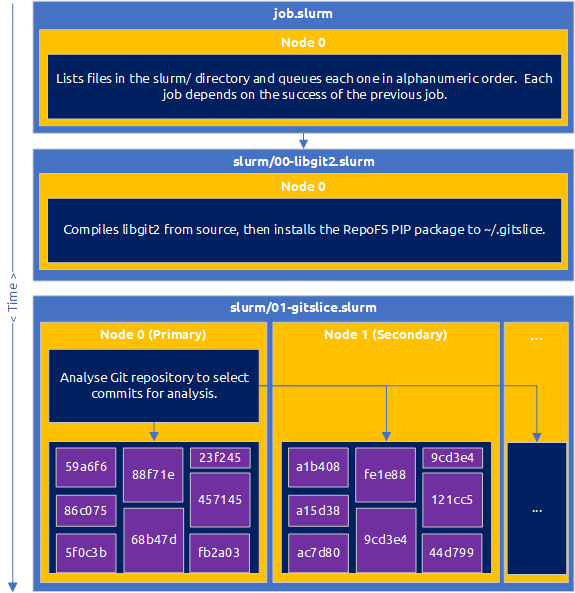
\includegraphics{slurm_overview}
        \caption{An overview of the SLURM jobs used.}
        \label{fig:slurm_overview}
    \end{figure}

    \subsection{Python script}
    \label{subsec:python-script}

    GitSlice uses the Python logging library for logging.
    There are 5 categories for logs:

    \begin{itemize}
        \item \codeword{DEBUG} (log level 10) contains information about precisely what GitSlice is doing, the values it receives for configuration options and the output generated by an analysis.
              This is an extremely verbose level and will produce large amounts of output - it is generally expected this is only used for debugging GitSlice.
        \item \codeword{INFO} (log level 20) contains some general information about the commits selected, and when executions are starting and are finished.
              This is the default level, and provides updates about what GitSlice is doing without producing an overwhelming amount of output.
        \item \codeword{WARNING} (log level 30) there are currently no warnings produced by GitSlice but if this log level was used, it would indicate conditions which might cause problems later but GitSlice is continuing as normal for now.
        \item \codeword{ERROR} (log level 40) this is a serious condition which will not necessarily stop GitSlice but is likely to be a serious problem and is highly likely to produce unreliable output.
              This primarily indicates that an analysis didn't complete with a \codeword{0} error code.
        \item \codeword{CRITICAL} (log level 50) includes critical errors mean that GitSlice has failed, and that execution will end imminently.
              This occurs if the filesystem cannot be brought up or if some other serious condition occurs that mean GitSlice cannot continue.
    \end{itemize}

    All instances of GitSlice will begin by retrieving the command-line options passed.
    Each instance then outputs some information about the system it is running on at level \codeword{DEBUG}.
    Each instance will then read the configuration file as given in the command-line arguments.
    This configuration file contains all the required information about the analysis GitSlice should perform.

    At this point the filesystem manager is started.
    This component is responsible for preparing (and at the end, deleting) the filesystem required for execution.
    When the filesystem manger is creating the requisite files this is known as bringing the filesystem up, and subsequently bringing it down refers to deleting temporary files and unmounting the filesystem.

    The filesystem manager has three tasks to bring the filesystem up: creating directories, cloning the repository and bringing the RepoFS mount up.
    Directories created include the temporary and output directories as well as the directory to contain the repository and the virtual filesystem.
    To bring up the RepoFS mount, a script called fsUp.sh is used.
    This script ensures the correct modules (specifically, Python and Git) are loaded, activates the virtual environment from the \codeword{00-libgit2.slurm} job and then invokes the RepoFS command to bring up a virtual filesystem representation of the repository.
    This script requires that the \codeword{00-libgit2.slurm} job completed successfully.
    
    \subsubsection{Tests}
    \label{subsubsec:tests}

    The \codeword{git-slice/} directory, which contains the Python code also contains unit tests for ensuring the correct operation of GitSlice.
    Unit tests have been written using the Python \codeword{Unittest} library which is provided as part of Python and as a result no additional packages need to be installed.
    Unit tests are run using the \codeword{pytest} package which provides code coverage information.
    Test files are named in the format \codeword{test_module.py}, for example tests for \codeword{main.py} live in \codeword{test_main.py}.
    Often Python projects will create a separate \codeword{tests/} directory but as there are only a few Python files, storing them in the same directory ensures they are easily found and can avoid issues with importing modules.
    Coverage reports for unit tests were generated as part of the CI/CD process, see \autoref{subsubsec:coverage}.

    End-to-end testing was performed locally and then on Kelvin, using the dry run mode to confirm the correct selection of commits for analysis.
    PyCharm, which was used to develop GitSlice provides a ``deployment'' feature which allows for files to be uploaded via SFTP to a remote server and for an SSH session to be opened within the IDE.
    When the application was validated locally, the files were uploaded to Kelvin and full analysis was run to confirm the correct operation of GitSlice.

    Static application security testing (SAST) was also performed during the CI/CD pipeline, more information on this can be found in \autoref{subsubsec:sast}.

    \subsubsection{Requirements files}
    \label{subsubsec:requirements-files}

    Text files are commonly used to define the required packages for Python applications, these usually follow a common format such as \codeword{test_requirements.txt}, \codeword{dev_requirements.txt} etc.
    GitSlice contains three requirements files used for different situations.
    
    \codeword{requirements.txt}: the \codeword{requirements.txt} file is the main requirements file and contains the required packages for running GitSlice.
    This is the requirements file which is used when running GitSlice on Kelvin---i.e. \codeword{python3 -m pip install -r requirements.txt} is run before executing the \codeword{git-slice/main.py} script.
    This file does not contain testing requirements such as \codeword{pytest} and \codeword{pytest-cov}.
    
    \codeword{test_requirements.txt}: the \codeword{test_requirements.txt} file is used for installing the packages required to run CI jobs such as coverage and linting tests.
    More information on CI jobs is provided in \autoref{subsec:ci/cd}.
    Importantly, this file doesn't contain requirements such as \codeword{torcpy} which will fail installation in CI because no MPI runner is available (such as OpenMPI).
    This is why an additional requirements file is required for CI\@.
    When developing GitSlice both the \codeword{requirements.txt} and \codeword{test_requirements.txt} files will be required.
    
    \codeword{misc_requirements.txt}: the \codeword{misc_requirements.txt} file contains packages required for running scripts in the \codeword{misc-scripts/} directory.
    These are primarily scripts for generating graphs on the GitSlice output, and they are not part of GitSlice itself and installing them on Kelvin when running GitSlice would therefore be unnecessary.
    More information on these scripts is given in \autoref{subsec:miscellaneous-scripts}.

    \subsubsection{Documentation}
    \label{subsubsec:documentation}

    All functions in GitSlice contain docstrings to describe the purpose of the function.
    Docstrings are string literals which are the first statement of a class or function in Python, automated tools can then be used to generate documentation from the docstrings.
    Each docstring contains a brief description of the functions along with the expected inputs and outputs.

    GitSlice uses Sphinx to generate its documentation.
    All documentation related files are stored within the \codeword{docs/} directory.
    There is a CI/CD job which builds a set of HTML files from the \codeword{docs/} directory.
    These HTML files are then published to GitLab pages and are available at~\cite{docs_site}.
    More information is on this process is provided in \autoref{subsec:ci/cd}.

    \subsection{Miscellaneous scripts}
    \label{subsec:miscellaneous-scripts}

    A \codeword{misc-scripts/} directory contains some additional scripts written in the development of GitSlice which are not a part of the main project.
    Specifically, it contains \codeword{parse_output.py} file which was used to generate graphs to visualise output from GitSlice, and later it was adapted to produce CSV files for loading into LaTeX to create graphs.

    The script reads from an output directory created by GitSlice, reading each file and looking for lines which match some search terms, when a line is found it attempts to pull data from this line.
    It does this by splitting a line at each space and producing a list---for example, \codeword{one two three} would produce \codeword{['one', 'two', 'three']}.
    The user is prompted at the start of the script for search terms and their list positions, for example searching for the line \codeword{100 tests run, 90 passed, 10 failed} the user would input \codeword{tests} at position \codeword{1}, \codeword{run,} at position \codeword{2}, \codeword{passed,} at position \codeword{4}.
    The user is also prompted to enter data points, this is the position of data points when a line matches---for example they would input \codeword{3} if they wanted to gather passed tests.
    Using the output filename which contains the time and date of the commit, it can use this information to produce time series information.
    The script then using these data points produces a graph over time and CSV file with the same data.

    \subsection{Version control}
    \label{subsec:version-control}

    Perhaps unsurprisingly, Git was used as the version control system during the development of GitSlice.
    Code was primarily pushed to my personal GitLab which is already configured with $2$ Docker runners to run CI/CD pipelines (see \autoref{subsec:ci/cd}).
    The repository was then pushed to the EEECS GitLab before submission therefore both these GitLab instances contain the same code.

    The IntelliJ ``.ignore'' plugin was used to generate a \codeword{.gitignore} file.
    This plugin provides pre-written ignore files for a large variety of languages, including Python.

    To track bugs during the development process, GitLab Issues was used.
    When fixing a bug, a topic branch named \codeword{issue-x} was created where \codeword{x} is the issue number from GitLab.
    When the bug was fixed, the branch was pushed and a merge request on GitLab was opened.
    Commit titles start with \codeword{[#x]} to denote the issue they relate two, again \codeword{x} is the issue number.
    When an issue was resolved, \codeword{Closes #x} was added to the merge request description and the merge request was accepted to close the issue via a merge request.
    A screenshot from GitLab Issues is shown in \autoref{fig:gitlab_issues}.

    \begin{figure}[h]
        \centering
        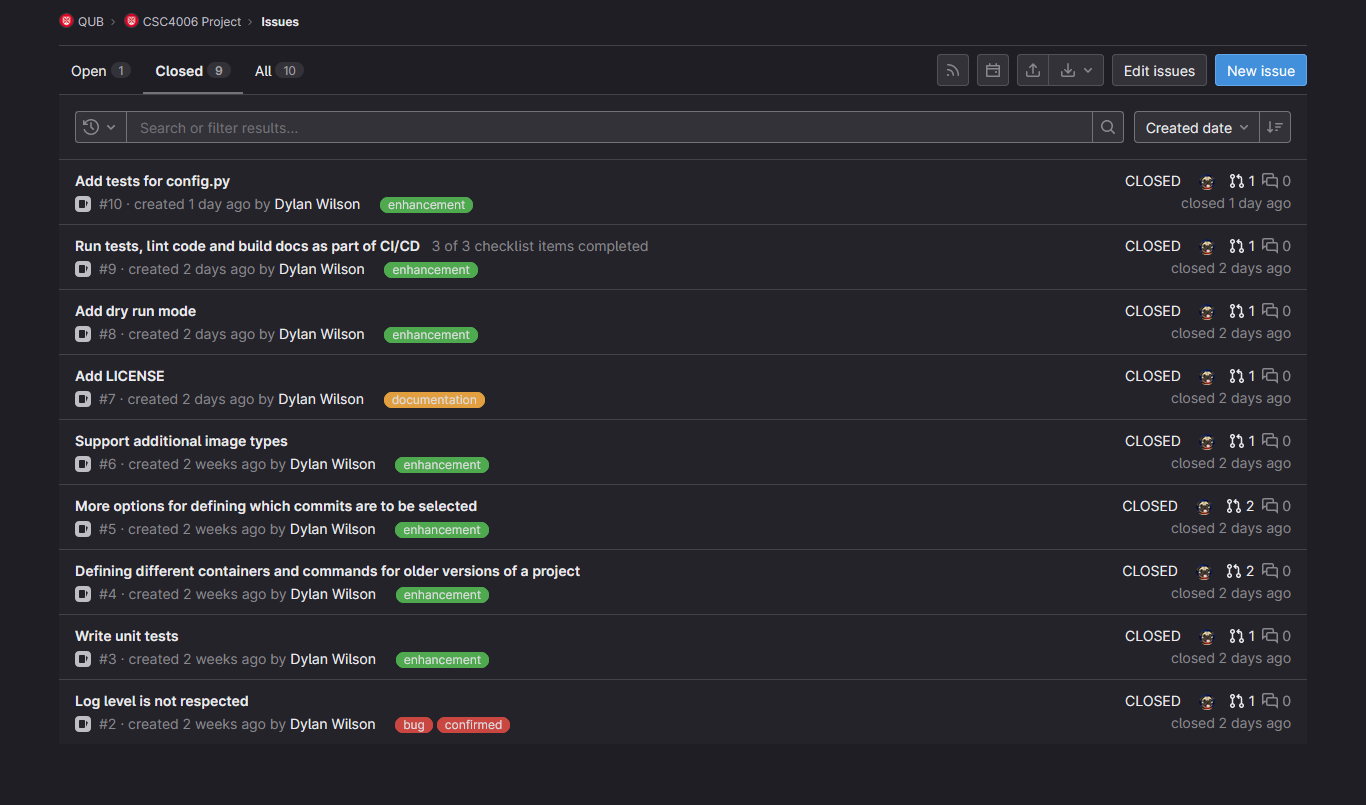
\includegraphics[width=\textwidth]{gitlab_issues}
        \vspace{-0.5cm}
        \caption[skip=0pt]{GitLab issues closed tab showing issues closed during development of GitSlice.}
        \label{fig:gitlab_issues}
    \end{figure}

    \subsection{CI/CD}
    \label{subsec:ci/cd}

    A \codeword{.gitlab-ci.yml} file is provided and contains multiple GitLab CI jobs for building, testing and deploying different parts of GitSlice.
    All jobs should run on a Docker runner (as opposed to, for example, a shell runner) as they define an image in which the script should be run.
    This file is designed to be portable, and it should be possible to push it to any GitLab repository with Docker runners without needing to update it (for example it uses the GitLab \codeword{\$CI\_REGISTRY\_IMAGE} variable instead of a hardcoded registry).

    \subsubsection{SAST Testing}
    \label{subsubsec:sast}

    GitLab provides static application security testing (SAST) out-of-the-box.
    GitLab provides a predefined \codeword{Security/SAST.gitlab-ci.yml} file which only requires a job called \codeword{sast} to be created.
    For Python projects GitLab uses Semgrep for SAST\@.
    When a warning is detected, a notice is displayed on the merge request and the full report can be downloaded.
    There were no security issues found during the development of GitSlice except outdated dependencies which have since been upgraded.

    \subsubsection{Docker images}

    As discussed in \autoref{subsubsec:singularity}, Docker containers can be used to run analysis on a commit and as discussed in \autoref{subsubsec:repofs}, \codeword{rsync} is required is the analysis needs to modify or create files.
    As such, the GitLab CI contains two jobs to build images with \codeword{rsync} available.
    The two jobs, \codeword{build-python} and \codeword{build-cloc} build Python and CLOC images respectively.
    CLOC is a simple Perl script for counting the total lines of code in an application.
    The \codeword{Dockerfile} for these images is stored in \codeword{docker/python/} and \codeword{docker/cloc/} respectively.

    The Python image is based on the Python image (Debian variant) and only adds \codeword{rsync}.
    The CLOC image is based on the Perl image (again, the Debian variant) downloads the CLOC Perl script and installs it as a system command (in \codeword{/usr/local/bin}).
    
    The script for building these containers is identical, and it is only the location of the \codeword{Dockerfile} which is different and as such as job, called \codeword{.docker-build} is provided.
    Jobs starting with \codeword{.} in GitLab are not built.
    This feature is useful for defining generalised jobs which can be extended by other jobs which can provide their own variables.
    The \codeword{.docker-build} job will build an image from the \codeword{Dockerfile} in the \codeword{\$DOCKER\_DIR} directory, this variable is then provided by the jobs which extend it.
    The image is named according to the \codeword{\$CONTAINER\_NAME} variable.

    The \codeword{build-python} and \codeword{build-cloc} jobs then extend the \codeword{.docker-build} job.
    This also allows for many images to be built by the \codeword{.gitlab-ci.yml} file relatively easily.
    
    It can take some time to build these containers, and they only need to be rebuilt when the \codeword{Dockerfile} changes and as such a \codeword{changes:} rule on the \codeword{.docker-build} job has been added meaning images are only rebuilt when the Dockerfile changes.

    \subsubsection{Linting}
    \label{subsubsec:linting}

    The Python code for GitSlice has been validated against PEP 8 (Python Enhancement Proposal 8) which describes the style guide for Python code.
    PyCharm was used to develop GitSlice and PEP 8 linting is provided out-of-the-box by PyCharm which provides warnings as code is being written.
    PyCharm also provides a reformat feature which can automatically fix code style problems.

    To enforce code quality standards in GitSlice during merge requests, the Flake8 Python linter is used to verify code style adherence as part of the CI/CD pipelines.
    This job is called \codeword{flake8} and is only run for merge requests.
    Most options have been left as their defaults except the \codeword{max-line-length} option.
    PEP 8 recommends lines are no longer than 79 characters which is often controversial as this is quite short and breaking lines at this point can often reduce readability instead of increasing it.
    This is often ignored by some projects---for example, the default \codeword{max-line-width} for PyCharm's PEP8 linting is \codeword{120} characters.
    As PyCharm was used for development of GitSlice, and it's code tidying feature by default uses \codeword{120} characters, a \codeword{.flake8} file is provided to override this value to \codeword{120}.

    \subsubsection{Unit test coverage}
    \label{subsubsec:coverage}

    The \codeword{coverage} job provides code coverage information is always run.
    GitLab provides as \codeword{coverage:} option for providing a regular expression to extract code coverage information.
    This value is this displayed in the GitLab UI and is useful for seeing code coverage at a glance, \autoref{fig:code_coverage_gitlab} shows this in a merge request (highlighted in yellow).

    \begin{figure}[h]
        \centering
        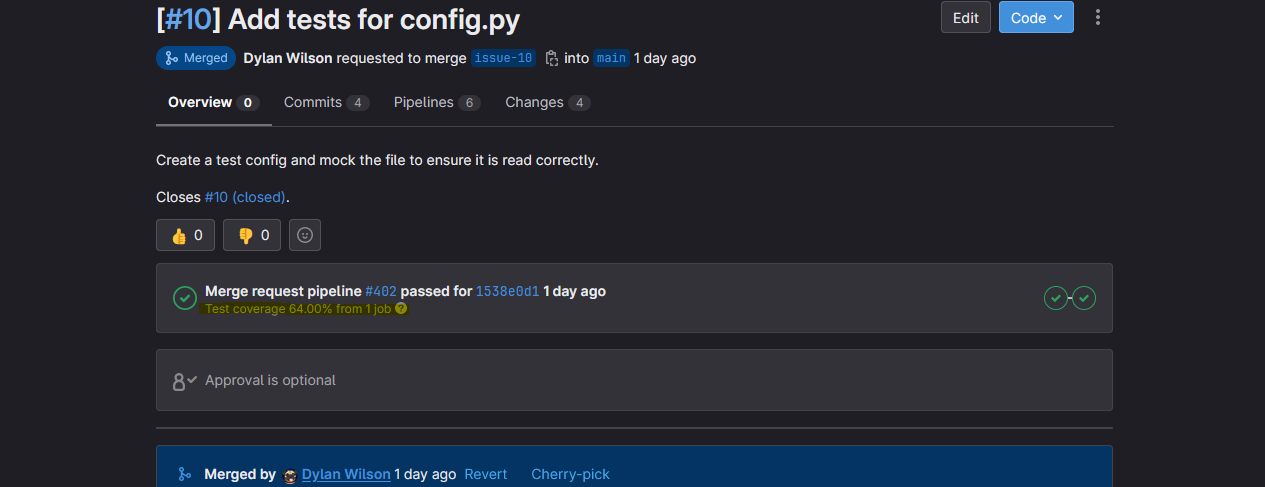
\includegraphics[width=\textwidth]{code_coverage_gitlab}
        \vspace{-0.5cm}
        \caption[skip=0pt]{Code coverage information shown in a merage request.}
        \label{fig:code_coverage_gitlab}
    \end{figure}

    Providing this information to GitLab allows for code coverage badges to be added to the \codeword{README.md} file to see code coverage information quickly---these badges are common in open source projects.
    It also allows for premium accounts to see how code coverage changes over time.
    Additionally, the coverage report is marked as an artifact which allows for GitLab to show which lines are covered by tests in merge requests.
    This job will fail when at least one test fails, allowing for rules such blocking merge requests until the coverage job completes successfully.
    These features are useful for the ongoing development of GitSlice as an open source project to ensure passing tests and to monitor code coverage.

    \subsubsection{Documentation}

    The \codeword{pages} job publishes the HTML documentation generated by Sphinx to GitLab pages.
    See \autoref{subsubsec:documentation} for information on how documentation is generated.
    This job is relatively simple, it simply installs packages from \codeword{test_requirements.txt} and runs Sphinx to generate documentation (as HTML files) in a directory called \codeword{public/} in the root of the GitSlice repository.
    A live version is available at~\cite{docs_site}.
    As noted in \autoref{subsec:ci/cd} this job is portable and will publish the documentation site on any GitLab instance which has GitLab Pages installed.

    \section{References}
    \label{sec:references}

    \bibliographystyle{plain} % We choose the "plain" reference style
    \bibliography{references} % Entries are in the refs.bib file

    \section{Appendices}
    \label{sec:appendices}

    \subsection{Appendix A: Sample configuration file}\label{subsec:appendix-a:-sample-configuration-file}

    \inputminted[bgcolor=bg,frame=lines,framesep=2mm,linenos]{yaml}{./listings/sample_config_cloc.yml}

\end{document}